\originalchapter{本科作业: 静电学}
本章按 8.07 官方作业1--5逐项整理. 题面采用数学等价的中文表述, 保留可取得的子问; 解答均为\textbf{AI 独立解答}, 未取得相应作业官方解答. 仅给商业教材题号的项目列在各节末尾, 不凭记忆补成所谓原题. 参考理论章节的已证结论时给出明确定位.

\originalsection{作业1}
\begin{exercise}
原题1 (20分). 以 $\epsilon_{ijk}$ 写叉积, 证明: (a) $\epsilon_{ijk}\epsilon_{inm}=\delta_{jn}\delta_{km}-\delta_{jm}\delta_{kn}$; (b) $\vct A\times(\vct B\times\vct C)=\vct B(\vct A\cdot\vct C)-\vct C(\vct A\cdot\vct B)$; (c) $\nabla\cdot(\vct A\times\vct B)=\vct B\cdot\nabla\times\vct A-\vct A\cdot\nabla\times\vct B$; (d) $\vct A\times(\nabla\times\vct A)=\frac12\nabla A^2-(\vct A\cdot\nabla)\vct A$; (e) $\nabla\times(\vct A\times\vct B)=(\vct B\cdot\nabla)\vct A-(\vct A\cdot\nabla)\vct B+\vct A\nabla\cdot\vct B-\vct B\nabla\cdot\vct A$.
\end{exercise}
\begin{solution}
(a) 若 $j=k$ 或 $n=m$, 两边皆零; 否则左边仅在 $(n,m)=(j,k)$ 或 $(k,j)$ 时非零, 值分别为1、$-1$, 与右边一致. (b) 缩并两个 $\epsilon$ 后得到 $B_iA_jC_j-C_iA_jB_j$. (c) 展开 $\partial_i(\epsilon_{ijk}A_jB_k)$ 并分别把两项按旋度重排, 得所需式. (d) 第 $i$ 分量为 $\epsilon_{ijk}A_j\epsilon_{k\ell m}\partial_\ell A_m=A_j\partial_iA_j-A_j\partial_jA_i$, 第一项是 $\partial_i(A_jA_j)/2$. (e) 第 $i$ 分量为 $\epsilon_{ijk}\partial_j(\epsilon_{k\ell m}A_\ell B_m)=\partial_j(A_iB_j-A_jB_i)$; 对两个乘积展开即得四项, 其中微分作用的对象保持不变.
\end{solution}
\begin{exercise}
原题3 (15分). 若 $A'_i=R_{ij}A_j$, (a) 证明保持任意向量长度要求 $R_{ij}R_{ik}=\delta_{jk}$; (b) 写出逆变换; (c) 用链式法则证明标量的梯度按矢量变换.
\end{exercise}
\begin{solution}
(a) $|\vct A'|^2=A_j(R^\mathsf TR)_{jk}A_k$. 对所有 $\vct A$ 等于 $A_jA_j$ 意味着对称矩阵 $R^\mathsf TR-I$ 的二次型恒零, 取基向量及两基向量之和分别确定对角及非对角分量均零. (b) 左乘 $R^\mathsf T$ 得 $A_i=R_{ji}A'_j$. (c) $x_j=R_{ij}x'_i$, 所以 $\partial V'/\partial x'_i=(\partial V/\partial x_j)R_{ij}$.
\end{solution}
\begin{exercise}
原题5 (20分). 对 $a>0$ 定义 $f_a=-1/(4\pi\sqrt{r^2+a^2})$. (a) 求 $g_a=\nabla^2f_a$ 并画其草图; (b) 证明全空间积分为1; (c) 验证 $r\ne0$ 时 $a\to0$ 的点态极限为0.
\end{exercise}
\begin{solution}
径向微分给 $f'_a=r/[4\pi(r^2+a^2)^{3/2}]$, 故 $g_a=3a^2/[4\pi(r^2+a^2)^{5/2}]$. 它在 $r=0$ 有有限最大值 $3/(4\pi a^3)$, 随 $r/a$ 单调下降. 积分可直接写成 $\int g_a\dd^3x=[r^3/(r^2+a^2)^{3/2}]_0^\infty=1$. 对固定非零 $r$, 分子趋零而分母趋 $r^5$, 因而点态极限为零. 真正的分布极限须对测试函数积分: 取 $r=au$, 归一化核的质量集中于原点, 将 $\varphi(au\nn)$ 的局部连续性与尾部小质量结合, 得极限 $\varphi(0)$; 不能先取点态极限再积分.
\end{solution}
\begin{center}
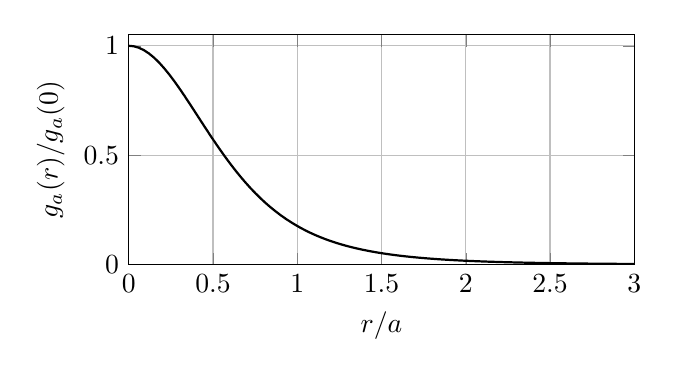
\begin{tikzpicture}
\begin{axis}[width=.66\textwidth,height=4.5cm,xlabel={$r/a$},ylabel={$g_a(r)/g_a(0)$},xmin=0,xmax=3,ymin=0,ymax=1.05,grid=major]
\addplot[thick,domain=0:3,samples=101] {(1+x^2)^(-2.5)};
\end{axis}
\end{tikzpicture}\par
作业1题5草图: 横纵坐标均无量纲, $a>0$.
\end{center}

\begin{exercise}
原题6 (10分). (a) 总电荷均为 $Q$、半径均为 $R$, 给出均匀带电球壳及位于 $xy$ 面圆环的体密度; (b) 写出柱坐标的三维狄拉克分布; (c) 半径 $b$ 的柱面每单位长度带电 $\lambda$, 写出体密度; (d) 求二维 $\nabla^2\ln s$.
\end{exercise}
\begin{solution}
(a) 球壳为 $Q\delta(r-R)/(4\pi R^2)$; 圆环为 $Q\delta(s-R)\delta(z)/(2\pi R)$. (b) 在 $s'>0$ 处为 $\delta(s-s')\delta_{2\pi}(\phi-\phi')\delta(z-z')/s$, 其中角度分布须按 $2\pi$ 周期解释; 轴线上坐标退化要直接用测试函数定义. (c) $\rho=\lambda\delta(s-b)/(2\pi b)$. (d) 原点外拉普拉斯为零, 小圆周通量为 $\oint\partial_s\ln s\dd l=2\pi$, 因而 $\nabla^2\ln s=2\pi\delta^{(2)}(\vct s)$.
\end{solution}
\begin{exercise}
原题7 (15分). 设闭曲面 $S=\partial V$, 开曲面边界为 $\Gamma$. 证明 (a) $\int_V\nabla\psi\dd^3x=\oint_S\psi\dd\vct a$ 并推出 $\oint_S\dd\vct a=0$; (b) $\int_V\nabla\times\vct A\dd^3x=-\oint_S\vct A\times\dd\vct a$; (c) $\int_S\nabla\psi\times\dd\vct a=-\oint_\Gamma\psi\dd\vct l$; (d) $\oint_S(\nabla\times\vct A)\cdot\dd\vct a=0$.
\end{exercise}
\begin{solution}
(a) 对常矢量 $\vct c$ 应用散度定理于 $\psi\vct c$, 得两边与任意 $\vct c$ 的点积相等. 取 $\psi=1$ 得附带结论. (b) 第 $i$ 分量由 $\int\epsilon_{ijk}\partial_jA_k=\oint\epsilon_{ijk}n_jA_k$ 得到, 交换 $j,k$ 后即为负叉积. (c) 对常矢量 $\vct c$ 用斯托克斯定理于 $\psi\vct c$, 因 $\nabla\times(\psi\vct c)=\nabla\psi\times\vct c$, 标量三重积重排给所需负号. (d) 散度定理及 $\nabla\cdot(\nabla\times\vct A)=0$ 给出. 各式要求场在积分域内充分光滑; 包含奇点时改用分布或挖洞处理.
\end{solution}
原题2只列 Griffiths 1.2、1.6; 原题4只列1.12及1.13(a), 无完整题面, 本稿不编造.

\originalsection{作业2}
\begin{exercise}
原题1 (15分). 令 $\bar\varphi(R)$ 为半径 $R$ 球面上 $\varphi$ 的平均值. (a) 对 $g=1/r-1/R$ 验证 $\int_{r<R}\nabla\cdot(g\nabla\varphi)=0$; (b) 展开散度; (c) 证明
$\varphi(0)-\bar\varphi(R)=-\frac1{4\pi}\int_{r<R}(1/r-1/R)\nabla^2\varphi\dd^3x$.
\end{exercise}
\begin{solution}
外边界 $g=0$; 内小球 $g\partial_r\varphi$ 的通量为 $O(a)$, 因而(a)成立. (b) 乘积法则为 $\nabla\cdot(g\nabla\varphi)=\nabla g\cdot\nabla\varphi+g\nabla^2\varphi$. (c) $\nabla g=-\hat{\rr}/r^2$, 第一项积分为 $-\int\dd\Omega\int_0^R\partial_r\varphi\dd r=4\pi[\varphi(0)-\bar\varphi(R)]$, 代回总积分为零即得结果. 调和函数的中心值等于球面平均值.
\end{solution}
\begin{exercise}
原题2 (10分). 同轴导体内外半径 $a,b$, 长度 $\ell$, 电荷 $+q,-q$. 忽略端效应, 求 (a) 场; (b) 外壳减内柱的电势差; (c) 电容及单位长度电容; (d) 小间隙极限.
\end{exercise}
\begin{solution}
第2章例题的高斯柱面通量为 $2\pi s\ell E_s=q/\eps$, 因而给 $\ee=q\hat{\vct s}/(2\pi\eps\ell s)$, $V_b-V_a=-q\ln(b/a)/(2\pi\eps\ell)$, $C=2\pi\eps\ell/\ln(b/a)$, $C'=C/\ell$. $b-a=d\ll a$ 时 $C\simeq\eps(2\pi a\ell)/d$. 电势差与电容所用正电压的符号区别在(b)中保留.
\end{solution}
\begin{exercise}
原题3 (15分). 半径 $R$ 的均匀带电实心球总电荷 $Q$. 求 (a) 场; (b) 无穷远为零的势; (c) 用场能积分求组装能; (d) 用 $\frac12\int\rho V$ 再算一次.
\end{exercise}
\begin{solution}
高斯定理给球内 $E_r=Qr/(4\pi\eps R^3)$, 球外 $E_r=Q/(4\pi\eps r^2)$. 由 $V(R)=Q/(4\pi\eps R)$ 向内积分, 得 $V_\mathrm{in}=Q(3-r^2/R^2)/(8\pi\eps R)$, 外势为 $Q/(4\pi\eps r)$. 场能分成内外:
\[
U_\mathrm{in}=2\pi\eps\int_0^R\left(\frac{Qr}{4\pi\eps R^3}\right)^2r^2\dd r=\frac{Q^2}{40\pi\eps R},\qquad
U_\mathrm{out}=2\pi\eps\int_R^\infty\left(\frac Q{4\pi\eps r^2}\right)^2r^2\dd r=\frac{Q^2}{8\pi\eps R},\qquad U=\frac{3Q^2}{20\pi\eps R}.
\]
另一算法用 $\rho=3Q/(4\pi R^3)$ 得
$U=2\pi\rho\int_0^R V_\mathrm{in}r^2\dd r=\rho Q[3R^3/3-R^3/5]/(4\eps R)$, 即同一结果.
\end{solution}
\begin{exercise}
原题4 (10分). 平行板面积 $A$, 间距 $d$, 用虚功分别在 (a) 电荷固定和 (b) 电压固定时求板间吸引力.
\end{exercise}
\begin{solution}
以 $d$ 增加为正方向. (a) $U=Q^2d/(2\eps A)$, 故 $F_d=-Q^2/(2\eps A)$. (b) 场能随 $d$ 增加而减少, 但电源功为 $V\dd Q$. 合势 $-\eps AV^2/(2d)$ 给 $F_d=-\eps AV^2/(2d^2)$. 两者以 $Q=CV$ 联系, 均为吸引.
\end{solution}
\begin{exercise}
原题5 (15分). $Q_i=C_{ij}V_j$. (a) 证明 $C_{ij}=C_{ji}$; (b) 对两个导体、$Q_1=-Q_2=Q$, 求通常的两端电容; (c) 求半径 $a<b$ 的同心球壳电容矩阵并核对两端电容.
\end{exercise}
\begin{solution}
(a) 第2章以调和基函数的梯度内积证明互易性, 也可先用不同组装次序证明逆电容矩阵对称. (b) 令 $D=C_{11}C_{22}-C_{12}^2$, 反演得 $V_1-V_2=Q(C_{11}+C_{22}+2C_{12})/D$, 所以 $C=D/(C_{11}+C_{22}+2C_{12})$. (c) 设 $C_s=4\pi\eps ab/(b-a)$, 外壳对无穷远的电容 $C_b=4\pi\eps b$. 有 $Q_1=C_s(V_1-V_2)$、$Q_1+Q_2=C_bV_2$, 故矩阵为 $\bigl(\begin{smallmatrix}C_s&-C_s\\-C_s&C_s+C_b\end{smallmatrix}\bigr)$. 代入(b)得 $C=C_s$.
\end{solution}
\begin{exercise}
原题7 (20分加分). 对光滑快速衰减测试函数, 求 $F[\varphi]=\int r^{-1}\nabla^2\varphi\dd^3x$, 从分布定义证明 $\nabla^2(1/r)=-4\pi\delta^3$.
\end{exercise}
\begin{solution}
命题\ref{prop:point}的挖洞计算完整给出 $F[\varphi]=-4\pi\varphi(0)$. 关键是内球面外法线为 $-\hat{\rr}$, 边界项中的 $-\varphi/a^2$ 留下有限值, 而被挖去体积与其余边界项趋零. 这证明对任意测试函数相等, 不是只核对一个总积分.
\end{solution}
原题6只列 Griffiths 2.48 的题号及解题提示, 缺少真空二极管条件与子问, 不作为已取得题面.

\originalsection{作业3}
\begin{exercise}
原题2 (15分). 接地 $xy$ 导体平面用半径 $a$ 的上半球凸起替换中心圆盘; 点电荷 $q$ 位于 $(0,0,z_0)$, $z_0>a$. 求镜像并证明吸引力大小为
$\frac1{4\pi\eps}[q^2/(4z_0^2)+4q^2a^3z_0^3/(z_0^4-a^4)^2]$.
\end{exercise}
\begin{solution}
放三个镜像: $-q$ 在 $-z_0$, $-qa/z_0$ 在 $a^2/z_0$, $+qa/z_0$ 在 $-a^2/z_0$. 平面上上下对应电荷抵消, 球面上每个外部电荷及其球内镜像抵消. 三镜像皆在导体内部或求解域外, 唯一性给出解. 对真实电荷求库仑力,
\[
F_z=-\frac{q^2}{4\pi\eps}\left[\frac1{4z_0^2}
+\frac a{z_0}\left(\frac1{(z_0-a^2/z_0)^2}-\frac1{(z_0+a^2/z_0)^2}\right)\right].
\]
通分后第二项为 $4a^3z_0^3/(z_0^4-a^4)^2$, 方向向下.
\end{solution}
\begin{exercise}
原题3 (15分), MIT 改编 sheet 注明基于 Jackson 2.11. 线电荷 $\lambda$ 平行于半径 $b$ 的导体柱轴, 距轴 $R>b$, 柱保持恒电势且远处电势为零. 求 (a) 镜像线电荷位置和大小; (b) 柱电势.
\end{exercise}
\begin{solution}
二维线势为 $-\lambda\ln d/(2\pi\eps)$ 加常数. 镜像 $-\lambda$ 位于同径向的 $b^2/R$, 写 $V=\lambda\ln(d_-/d_+)/(2\pi\eps)$, 远处距离比趋1. 柱面上 $d_+/d_-=R/b$, 故 $V_0=\lambda\ln(b/R)/(2\pi\eps)$. 远处零势条件排除了另加轴上线电荷的净对数项. 本题保留 MIT 实际给出的改编陈述, 不另外补入商业原书题面.
\end{solution}
\begin{exercise}
原题4 (20分). 单导体以无穷远为零, 电容 $Q=CV_0$. (a) 证明 $C=\eps V_0^{-2}\int|\nabla V|^2\dd^3x$; (b) 对任意同边界试探势 $\Psi$ 证明其梯度能给电容上界; (c) 证明被另一导体包围的较小导体电容较小; (d) 给边长 $a$ 的立方体电容界, 与原题给出的 $0.661(4\pi\eps a)$ 比较.
\end{exercise}
\begin{solution}
(a) 场能等于 $CV_0^2/2$. (b) 写 $\Psi=V+u$, $u$ 在边界为零. 交叉项 $\int\nabla V\cdot\nabla u=0$, 故试探梯度能为真实能加非负的 $\int|\nabla u|^2$. (c) 把电势归一成1, 在导体内部延拓为常数. 较大导体要求试探函数在更大的区域为1, 容许类更小, 能量下确界更大. 对严格包含且新增区域实际存在非零场, 不等式严格. (d) 立方体内切与外接球半径分别为 $a/2$、$\sqrt3a/2$, 故
$\frac12(4\pi\eps a)<C_\mathrm{cube}<\frac{\sqrt3}2(4\pi\eps a)$. 给定的0.661位于0.5与0.866之间, 与界一致; 数值不是本稿独立计算值.
\end{solution}
原题1和5分别只列 Griffiths 3.8、3.15, 不补题面.

\originalsection{作业4}
\begin{exercise}
原题2 (25分). 半径 $R$ 的导体球中心在 $z_0>R$, 球势 $V_0$, 下方 $xy$ 平面接地. 初始中心电荷 $q_0=4\pi\eps RV_0$. (a) 加首个平面镜像; (b) 再交替修正球面与平面, 求直到第四个新增镜像的位置和电荷; (c) 求此时球面势; (d) 写出对应前几项的总静电能级数; (e) 将实心球改为空壳是否改变外场?
\end{exercise}
\begin{solution}
令球内正电荷 $q_n$ 位于 $z_n$, $z_0$ 为初始位置. 每个 $q_n$ 有平面镜像 $-q_n$ 在 $-z_n$, 而该负电荷的球镜像为
\[
q_{n+1}=\frac{Rq_n}{z_0+z_n},\qquad z_{n+1}=z_0-\frac{R^2}{z_0+z_n}.
\]
所以依次新增 $-q_0$, $q_1=q_0R/(2z_0)$, $-q_1$, $q_2=q_0R^2/(4z_0^2-R^2)$; $z_1=z_0-R^2/(2z_0)$, $z_2=z_0-2z_0R^2/(4z_0^2-R^2)$. 球面上每个 $-q_n$ 和 $q_{n+1}$ 的势相消, 初始电荷留下 $V_0$. 有限截断到 $q_2$ 时球面仍等势, 平面还残留最后一项, 只有无穷级数同时满足两边界. 精确能量为
$U=\frac12V_0\sum_{n\ge0}q_n=\frac12V_0q_0[1+R/(2z_0)+R^2/(4z_0^2-R^2)+\cdots]$.
在空壳内部没有额外电荷的条件下, 外部边界和总求解域相同, 外场不变.
\end{solution}
\begin{exercise}
原题3 (15分), MIT sheet 注明改编自 Jackson 3.5. 球腔半径 $a$, 表面给定 $V_0(\theta,\phi)$. 证明球内势可按 $(r/a)^\ell Y_{\ell m}$ 展开并求系数.
\end{exercise}
\begin{solution}
第3章的径向方程有 $r^\ell,r^{-\ell-1}$ 两支, 原点正则排除后者. 因球谐函数正交, 系数是 $A_{\ell m}=\int Y_{\ell m}^*V_0\dd\Omega$. 对足够光滑的边界, 该级数在球内收敛并满足调和方程, 唯一性确定解; 对分段边界按内部极限解释.
\end{solution}
原题1、4、5、6只列 Griffiths 3.15、3.20、3.22、3.41. 原题1与作业3的同一教材引用重复, 不当作新增已获题面.

\originalsection{作业5}
\begin{exercise}
原题2 (20分), MIT sheet 注明基于 Jackson 3.3. 半径 $R$ 的薄导体圆盘在 $xy$ 面, 势为 $V_0$. 已知面密度与 $(R^2-s^2)^{-1/2}$ 成正比. (a) 推导 $r>R$ 的勒让德势级数; (b) 求电容.
\end{exercise}
\begin{solution}
用 $\sigma=K/\sqrt{R^2-s^2}$ 表示两面的合计密度. 轴线势为
\[
V(z)=\frac K{2\eps}\int_0^R\frac{s\dd s}{\sqrt{R^2-s^2}\sqrt{s^2+z^2}}
=\frac K{2\eps}\arctan\frac R{|z|}.
\]
第二个等号用 $u=\sqrt{R^2-s^2}$ 后积分 $\int_0^R\dd u/\sqrt{R^2+z^2-u^2}$. 在 $z=0$ 得 $K=4\eps V_0/\pi$. 对 $z>R$, $\arctan(R/z)=\sum_{\ell\ge0}(-1)^\ell(R/z)^{2\ell+1}/(2\ell+1)$. 轴对称且关于赤道对称, 每项外部调和延拓为 $r^{-2\ell-1}P_{2\ell}(\cos\theta)$, 故
\[
V(r,\theta)=\frac{2V_0R}{\pi r}\sum_{\ell=0}^\infty\frac{(-1)^\ell}{2\ell+1}
(R/r)^{2\ell}P_{2\ell}(\cos\theta).
\]
总电荷 $Q=2\pi K\int_0^Rs\dd s/\sqrt{R^2-s^2}=2\pi KR=8\eps RV_0$, 所以 $C=8\eps R$.
\end{solution}
\begin{exercise}
原题4 (20分). 用无迹对称张量与 $\hat{\vct u}_+=(\hat{\vct x}+i\hat{\vct y})/\sqrt2$ 构造球谐: (a) 求 $Y_{31}$; (b) 求任意 $\ell$ 的 $Y_{\ell\ell}$; (c) 由四阶无迹张量求 $P_4(\cos\theta)$. 采用原题的构造: 对 $m\ge0$, 取
\[
 C^{(\ell,m)}=d_{\ell m}\{\vct u_+^{\otimes m}\hat{\vct z}^{\otimes(\ell-m)}\},\quad
 d_{\ell m}=\frac{(-1)^m(2\ell)!}{2^\ell\ell!}
 \sqrt{\frac{2^m(2\ell+1)}{4\pi(\ell+m)!(\ell-m)!}}.
\]
花括号表示完全对称化再去迹, $Y_{\ell m}=C^{(\ell,m)}_{i_1\cdots i_\ell}n_{i_1}\cdots n_{i_\ell}$; 负 $m$ 用 $Y_{\ell,-m}=(-1)^mY_{\ell m}^*$ 定义. 此约定含 Condon--Shortley 相位并使 $\int|Y_{\ell m}|^2\dd\Omega=1$.
\end{exercise}
\begin{solution}
(a) 三阶投影 $n_in_jn_k-(n_i\delta_{jk}+n_j\delta_{ik}+n_k\delta_{ij})/5$ 与 $u_{+i}z_jz_k$ 收缩给 $(\vct u_+\cdot\nn)(\cos^2\theta-1/5)$. 原题归一化常数给
$Y_{31}=-\sqrt{21/(64\pi)}(5\cos^2\theta-1)\sin\theta e^{i\phi}$.
(b) 因 $\vct u_+\cdot\vct u_+=0$, 全部 $\vct u_+$ 的乘积已经无迹; 收缩给 $2^{-\ell/2}\sin^\ell\theta e^{i\ell\phi}$. 设$I_\ell=\int_0^\pi\sin^{2\ell+1}\theta\dd\theta$, 分部积分给$I_\ell=2\ell I_{\ell-1}/(2\ell+1)$、$I_0=2$, 所以$\int\sin^{2\ell}\theta\dd\Omega=2\pi I_\ell=2^{2\ell+2}\pi(\ell!)^2/(2\ell+1)!$. 令此积分乘系数模平方为1, 便得
$Y_{\ell\ell}=(-1)^\ell\sqrt{(2\ell+1)!/(4\pi)}\sin^\ell\theta e^{i\ell\phi}/(2^\ell\ell!)$.
(c) 设四阶投影$n_in_jn_kn_l-a\sum_6\delta_{ij}n_kn_l+b\sum_3\delta_{ij}\delta_{kl}$. 对$i,j$取迹: 六项和变为$7n_kn_l+\delta_{kl}$, 三项和变为$5\delta_{kl}$, 所以$1-7a=0$、$-a+5b=0$, 即$a=1/7,b=1/35$. 因而四阶无迹投影是 $n_in_jn_kn_l-\frac17\sum_6\delta_{ij}n_kn_l+\frac1{35}\sum_3\delta_{ij}\delta_{kl}$. 与四个 $z$ 收缩得到 $x^4-6x^2/7+3/35$, $x=\cos\theta$. 乘原题给的 $(8)!/[2^4(4!)^2]=35/8$, 得 $P_4(x)=(35x^4-30x^2+3)/8$.
\end{solution}
\begin{exercise}
原题5(c), 10分加分. 将 $V_\mathrm{dip}=\pp\cdot\nn/(4\pi\eps r^2)$ 作为分布, 通过测试函数、挖去小球和分部积分, 推导包含接触项的电场.
\end{exercise}
\begin{solution}
令 $T_i=x_i/r^3$. 第4章已对任意测试函数证明 $\partial_jT_i=\PV(\delta_{ij}-3n_in_j)/r^3+(4\pi/3)\delta_{ij}\delta^3$. 因 $V=p_iT_i/(4\pi\eps)$, 取负梯度得 $\ee=\PV[3(\pp\cdot\nn)\nn-\pp]/(4\pi\eps r^3)-\pp\delta^3/(3\eps)$. 被挖去体积的 $T_i\partial_j\varphi$ 为 $O(a)$, 内表面积分趋于 $4\pi\delta_{ij}\varphi(0)/3$, 这是接触项的来源.
\end{solution}
原题1、3和5(a)--(b)只引用 Griffiths 3.22、3.45、3.42, 无完整商业题面; 5(c)是 MIT 完整给出的追加题, 与缺失部分分开记载.
